\documentclass{article}
\usepackage[utf8]{inputenc}
\usepackage{graphicx}
\usepackage{amsmath}
\usepackage{xurl}

\title{Recurrent model for Graph Network: an application to the World Trade Network dataset}
\author{Lorenzo Jacopo Pileggi}
\date{September 2022}

\begin{document}

\maketitle

\section{Introduction}
We extended the functionalities of graph\_nets to cope with temporal graph data, and applied such framework to the World Trade Network dataset to make predictions on countries' GDP trends, comparing them to the ones of a simple RNN model on GDP data only.

\section{Data preprocessing}
The data relative to the World Trade Network come from the UN comtrade database: \url{https://comtrade.un.org/}, whereas yearly GDP figures are taken from \url{https://public.knoema.com/mhrzolg/historical-gdp-by-country-statistics-from-the-world-bank-1960-2019}; both of them are measured in USD.

From the former, we took the csv files relative to each country's trade figures in a given year, covering the period 1996-2018. From them we extracted the yearly aggregated volumes of exchanges between couples of countries, and then built a weighted adjacency matrix by averaging the figures of pairs of partner countries, as they usually differ, discarding values below 1 million USD. Finally, to ignore effects linked to inflation and growth of total global trade, we normalised both the trade and GDP data to make their sum equal to 1 for each year considered.

The adjacency matrix has been evaluated both through CPU and GPU computing to test the differences in performances: the former yielded the matrix in 22 s, the latter in 2.1 s.

\section{Description of the framework}
Our model is based on the GraphNetwork module of graph\_nets, implementing message-passing between different blocks (EdgeBlock, NodeBlock and GlobalBlock) through a reducer function, taking the information coming from different blocks and reducing it to add additional features to be used by the block in question. The Edge and NodeBlocks are provided with a recurrent model, made of a first MLP layer and a recurrent layer on top of it, using a GRU.

The node/edge tensors have to be of shape (n\_nodes/edges, n\_time\_steps, n\_features), with n\_features given by the combination of features relative to the corresponding layer, plus the ones yielded by the pooling operation. For the edge block, the receiver and sender nodes' values are taken, so that n\_features = 3 for edges. For the node block, the reducer function consists of taking the list of in- or out-going edges of a node and, given a number $n$, taking the $n$ sums of all the elements of such list whose index $i$ satisfies $i \mod{n} = k, k \in \{0, n-1\}$; since this is done for both in- and out-going edges, we end up with $2n + 1$ final features. The output of the last layer has then to be normalised to make the year-by-year sums equal 1, as our original data.

The competing model is analogous to the GraphIndependent module found in the graph\_nets modules: it consists of a GRU applied to the node and edge feature lists, without any pooling.

\section{Results and analyses}
 The simple GRU has been trained for 100 epochs, both for nodes and edges, whilst the Recurrent Graph Network, due to the high computational cost (around 6 minutes per epoch), only for 10; the rest of the parameters are found in Table ($\ref{tab:conf}$). In particular for the latter, the "pool dimension", i.e. the number of features added by the reducer function, has been set to 3, so that, for what we already said, n\_features = 7 for nodes.
 
 The training and validation set was fixed to the data from 1996 to 2011, and the test set to the remaining years. The optimiser has been chosen as Adam, and the loss function was taken as the mean squared error of predicted vs real streaks.

The final loss on the test set yielded by the RecGraphNetwork model resulted in $2.8824 \cdot 10^{-6}$, outperforming the simple GRU, with a loss of $3.3797 \cdot 10^{-6}$, testifying the validity of the novel approach. In Figure ($\ref{fig:1}$) and ($\ref{fig:2}$) are showed the plots of real data vs prediction for both the GRU and RecGraphNetwork, where we can see that, despite the better overall performances, the output of RecGraphNetwork turns out to be less accurate for time series values below $10^{-3}$, while the simple GRU keeps its accuracy even down to these orders of magnitude.

\section{Conclusions}
We tested the novel RecGraphNetwork framework on the World Trade Network and yearly GDP data, comparing the results with a simple recurrent model without message-passing. The overall results of the former turned out to be at par with our reference model, though more unstable for lower orders of magnitude.

\begin{table}[h]
\centering
  \begin{tabular}{lccccc}
    \hline
     model & \#n epochs & \#e epochs & n l rate & e l rate & pool dim\\
    \hline
     Simple GRU & 100 & 100 & 1e-4 & 1 & N/A \\
     RecGraphNetwork & 10 & 10 & 1e-4 & 1e-3 & 3\\
    \hline
\end{tabular}
  \caption{Config parameters of simple GRU and RecGraphNetwork.}
  \label{tab:conf}
\end{table}

\begin{figure}
    \centering
    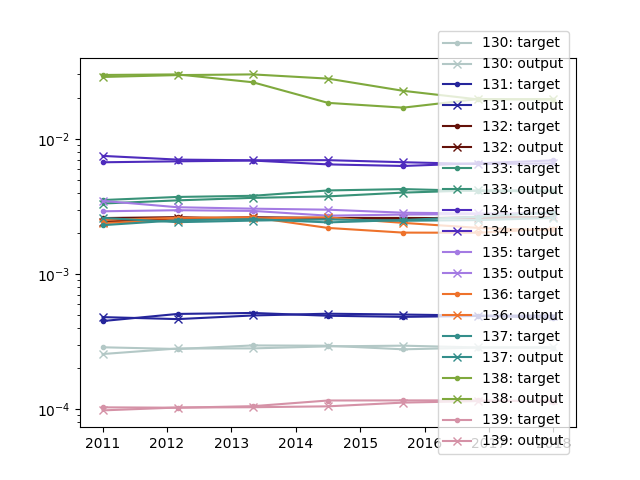
\includegraphics[width=100mm]{simple_output_13.png}
    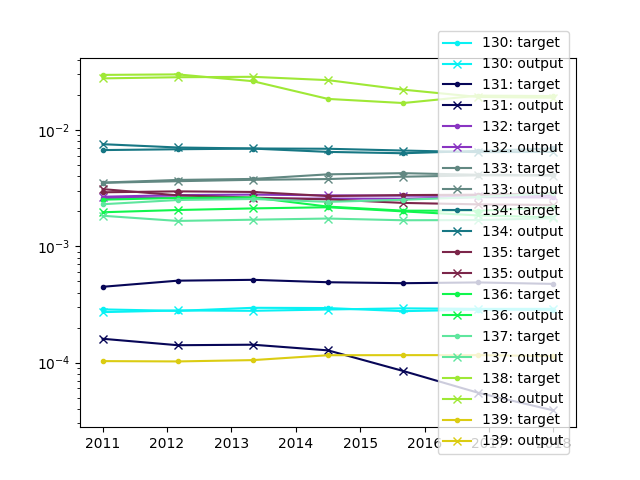
\includegraphics[width=100mm]{multi_output_13.png}
    \caption{Plots of real (dotted points) vs predicted series (crossed points) of simple GRU (upper plot) and RecGraphNetwork (lower plot), corresponding to the following countries (from 130 to 139): Papua New Guinea, Paraguay, Peru, Philippines, Poland, Portugal, Qatar, Romania, Russia, Rwanda. The discrepancy between the two model emerges below $10^{-3}$.}
    \label{fig:1}
\end{figure}

\begin{figure}
    \centering
    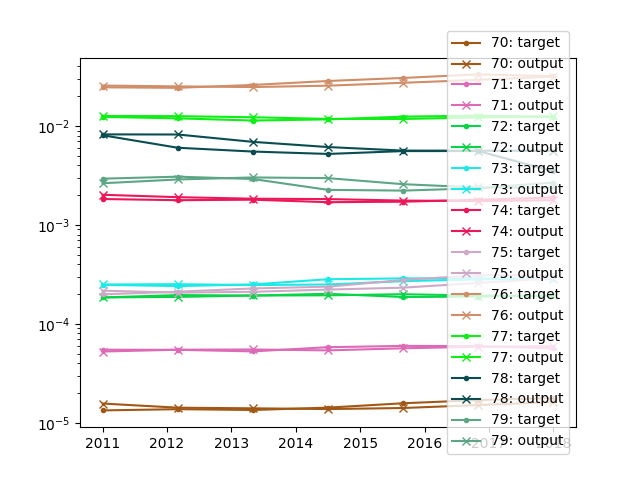
\includegraphics[width=100mm]{simple_output_7.png}
    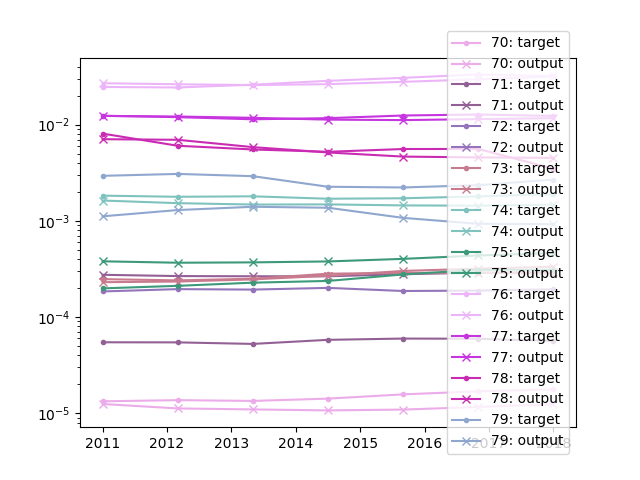
\includegraphics[width=100mm]{multi_output_7.png}
    \caption{Plots of real (dotted points) vs predicted series (crossed points) of simple GRU (upper plot) and RecGraphNetwork (lower plot), corresponding to the following countries (from 70 to 79): Guinea Bissau, Guyana, Haiti, Honduras, Hungary, Iceland, India, Indonesia, Iran, Iraq.}
    \label{fig:2}
\end{figure}

\end{document}
